With our background in both machine learning and \todo{medical background} we can now look at how we want to solve the problems associated with setting up a system for medical diagnosis.  
We will first look at the language and packages used in the creation of this thesis. We will go in depth into the reasoning behind why we chose the tools and packages that became the foundation of the programs. 

Then we will look at the setup of the complete program. Here we will go in-depth into both the different preprocessing algorithms, and take a look at the transfer learning network used during classifying.


\section{Libraries} 
In this chapter, we will discuss the foundation of our code, important external libraries, and the setup and execution of our project.  
We will first discuss the programming language in question, give insight into the reasoning behind it. Then we will look into the framework used for machine learning, and in detail how it implemented in our programming language. Lastly, we will look into the wrapper we use to get a higher level of abstraction over our code, together with custom wrapper functions that are used by our wrapper. 

\subsection{python}
When doing machine learning, the most popular languages, in no particular order, are Python, Java, R, C++, and C \todo{cite}. Some of these languages, like C and C++, are chosen for their speed, which is often a significant factor in Machine learning. Other languages, like R, is chosen because of its integration into the scientific community long before machine learning became a trend. The last group, consisting of Java and Python has gained popularity because of its already big user base and user-friendliness. Python is also the winner when it comes to machine learning because of, like R, its integration into the scientific community. 
Right now Python is the leading language for machine learning. Driven by this, there is considerable focus into making it faster, to compete with already fast languages, like the C family. 

Python is an interpreted, high-level, general-purpose programming language created in 1991.   It, like many other modern languages, is object-oriented and supports functional programming. 

Mainly because of the excellent support when it comes to machine learning, and the general "easy to use and no compiling" we have chosen python as the base for our code in this thesis. 



\subsection{tensorflow}
Arguably the biggest reason for the success of machine learning in python lies in Tensorflow.\todo{cite} Tensorflow is a machine learning package developed by Google in \todo{year} and has since then become the leading framework for machine learning worldwide \todo{cote}.  
Tensorflow is in use by companies like AMD, Nvidia, eBay and Snapchat. 


\todo{something about projects with python, and how may uses}

Tensorflow is today a multi-language tool, but it had its origin in python. It is just in later years that other languages have gotten tensorflow support.  
The data flows through a graph network, where the objects in the graph describe the mathematical operations used in the machine learning, and the edges between graphs are the multidimensional arrays storing the weights associated with the operation in question. The name Tensorflow is a combination of the flow we experience during calculation and the tensors between the mathematical operations. 

As stated, Python, and subsequently machine learning in Python, would be much slower than a counterpart in C. Because of this, Tensorflow works as a layer of abstraction to code running in the C language. 
 
\todo{cpu vs gpu}
\todo{, CNTK, or Theano}



\subsection{keras}
One of the least attractive things with tensorflow is its unnecessary complexity.  Even though Tensorflow offers more abstraction compared to running the code in pure C, the Tensorflow library can be unnecessarily complex.
As a result of this, many external libraries try to simplify many of the complexities that accompany tensorflow. 
Libraries like TFlearn was made as a modular and transparent deep learning library on top of tensorflow. It gives a higher-level API to Tensoflow to reduce complexity and speed up experiments. \todo{cite TFLEARN}
The most successful library for on top of Tensorflow is Keras \todo{cite keras}. 
Just as TFlearn, Keras is a high-level package written in python. It is capable of running on top of TensorFlow, CNTK, or Theano, which is the tree most popular machine learning libraries at this time. 
From their website they state that their four goals when creating Kears were:
\textbf{User friendliness. }\\
\textbf{Modularity. }\\
\textbf{Easy extensibility.}\\ 
\textbf{Work with Python. }\\

One of the core elements of Keras that makes it a better choice than just running, for instance, Tensorflow, is the concept of a model. A model in Keras is a way to organise the layers of the network in a more organised way, giving a better understanding of how the network is set up, and how each layer type contributes to the graph. \todo{more}

This thesis relies on Keras as a wrapper for tensorflow. As stated, the use of models and the simplicity of the language makes it an excellent choice of such a large project. Also, Keras has good support for convolutional operations which is the most used methods when managing images. Keras also has the most popular pretrained convolutional neural network models available in its package. \textit{Since one of our primary goal is to see how well our datasets generalise to the real world, transfer-learning will be a great tool to forgo unnecessary training}




\subsection{Custom functions for Keras, tensorflow and python}
\subsubsection{CWFC layer}
\subsubsection{Spectral conv?}
\subsubsection{Masklaod}
\subsubsection{self attention}
\subsubsection{masked loss}
\subsubsection{subpixel}
    
\subsection{Additional packs in Keras made by me}

\section{Design of the inpainting experiments}
When inpainting we have multiple hypotheses we want to test to see how it affects the results. We first want to set up a platform where every dataset is made with the same parameters, except for the dataset-specific parameters that define the dataset. Based on the hardware limitations \todo{more}

When generating the datasets, we use the Kvasir dataset as a base exclusively. When using only the Kvasir dataset, we have the CVC sets for testing. This selection of image source was made intentionally to have a fundamentally different test and training set, and the more differences between testing and training set the more of an indication of generalisation. 

\begin{figure}
     \centering
     \begin{subfigure}[b]{0.6\textwidth}
         \centering
         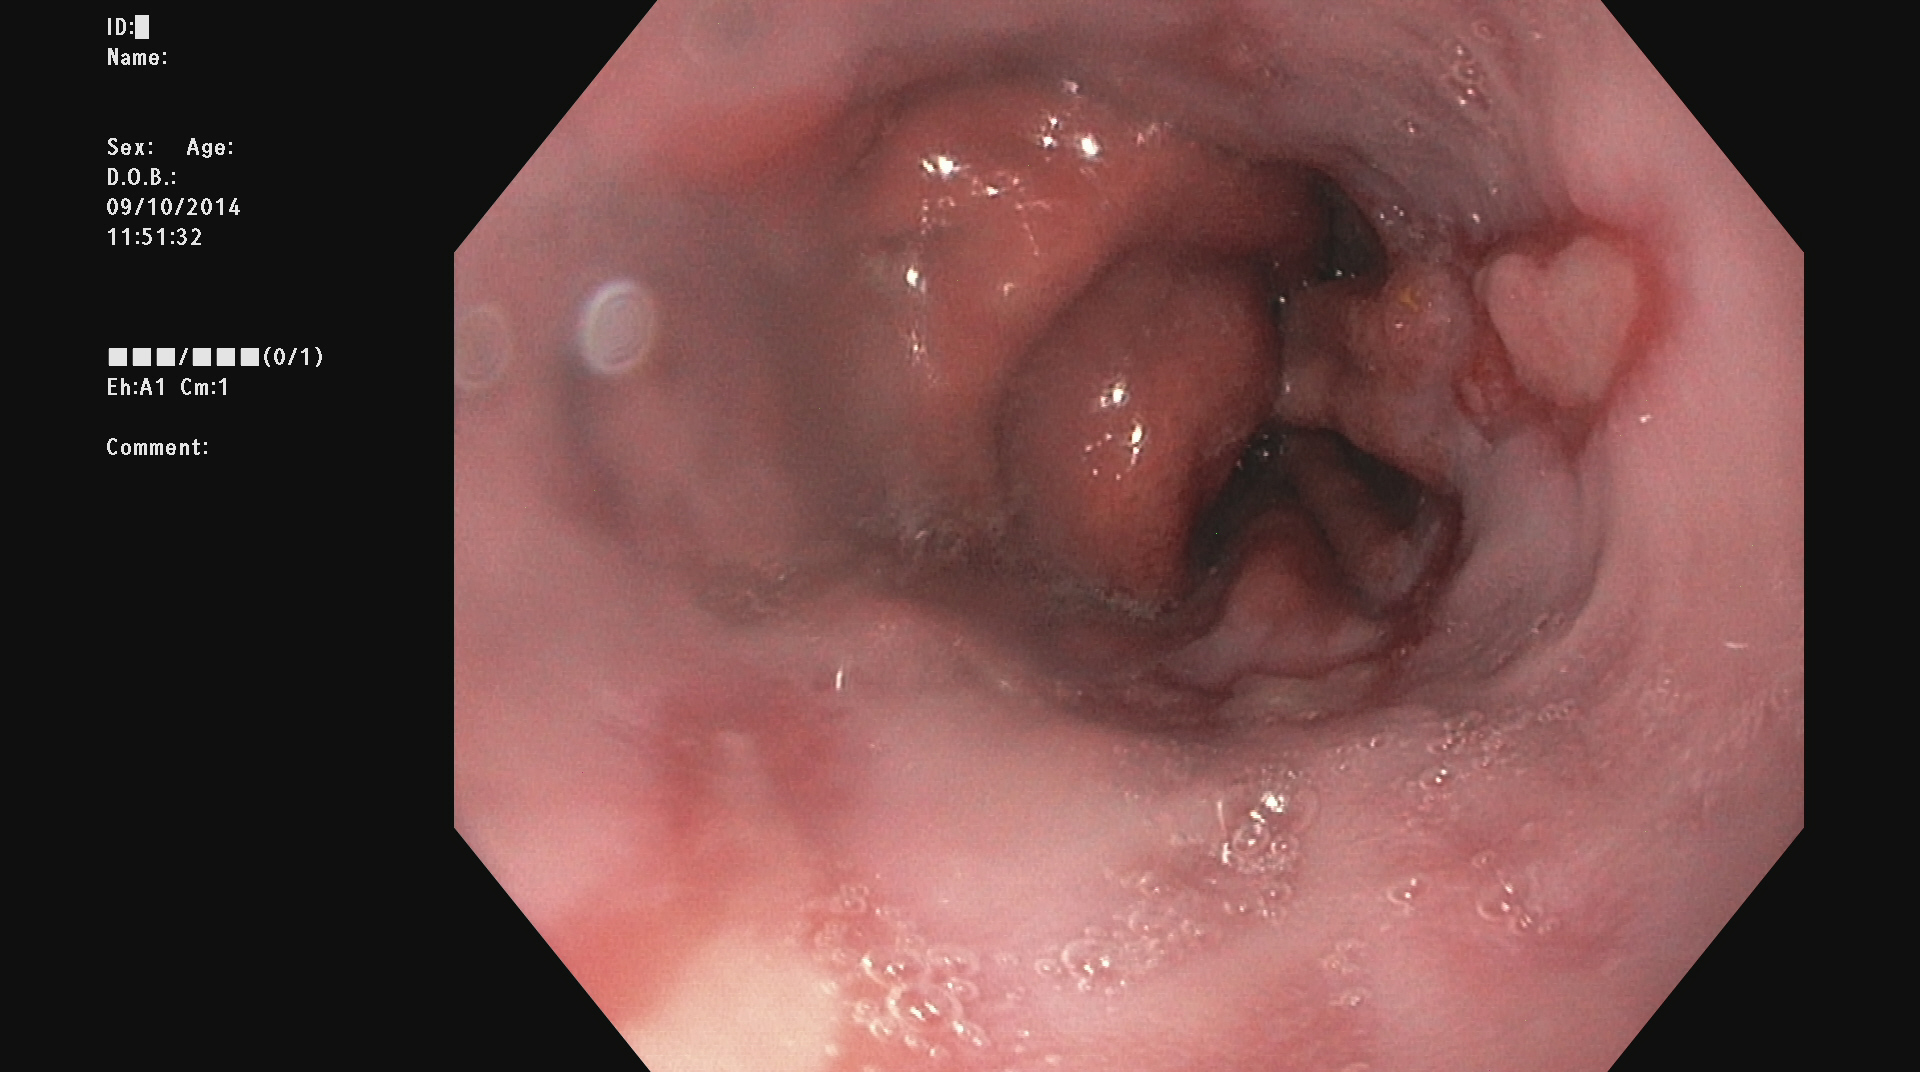
\includegraphics[width=\textwidth]{experiments/figures/leftframe.jpg}
         \caption{$y=x$}
         \label{fig:y equals x}
     \end{subfigure}
     \hfill
     \begin{subfigure}[b]{0.6\textwidth}
         \centering
         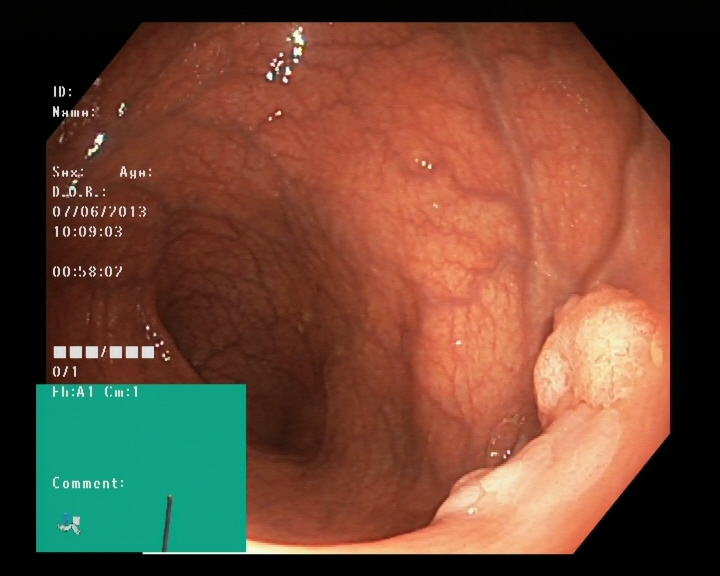
\includegraphics[width=\textwidth]{experiments/figures/greenframe.jpg}
         \caption{$y=3sinx$}
         \label{fig:three sin x}
     \end{subfigure}
        \caption{Three simple graphs}
        \label{fig:three graphs}
\end{figure}

Figure \todo{ref} shows three different image types from the Kvasir dataset. 
Image (a) shows the image class esophagitis. This image shows one of the main problems with the Kvasir dataset when it comes to dataset specific artefacts. In addition to the cut corners, we have an extra wide area to the left of the image containing non-relevant information like name, sex, and other comments. We can recall from chapter \todo{find where} that the area to the left does not contain any relevant information for the classification and subsequently can only give false information during classification. 
Another example of dataset-specific artefacts is in the image (b). In this image, we have the same cut corners as in most colonoscopy images. However, we also have an additional green square in the bottom left corner.

\begin{figure}
     \centering
     \begin{subfigure}[b]{0.5\textwidth}
         \centering
         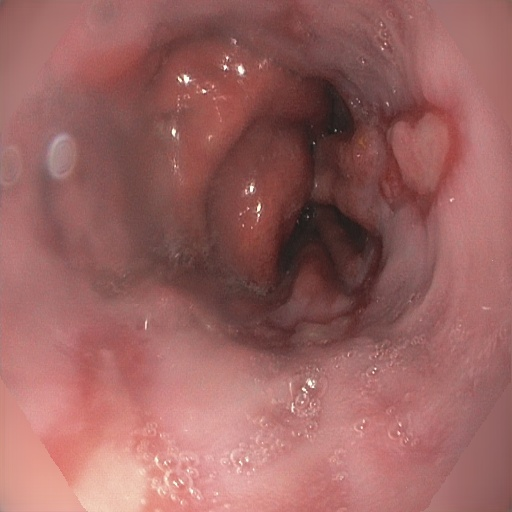
\includegraphics[width=\textwidth]{experiments/figures/noleftframe.jpg}
         \caption{$y=x$}
         \label{fig:y equals x}
     \end{subfigure}
     \hfill
     \begin{subfigure}[b]{0.5\textwidth}
         \centering
         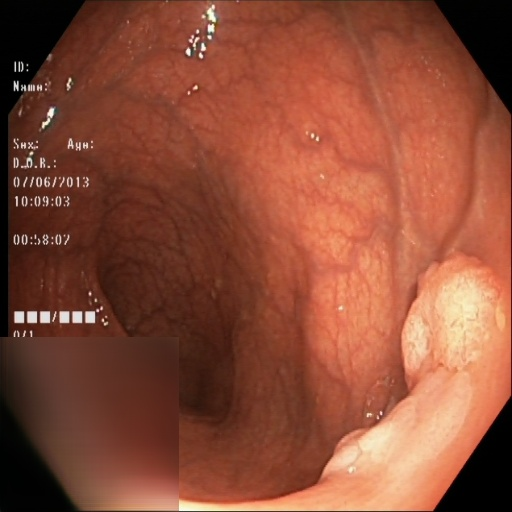
\includegraphics[width=\textwidth]{experiments/figures/nogreenframe.jpg}
         \caption{$y=3sinx$}
         \label{fig:three sin x}
     \end{subfigure}
        \caption{Three simple graphs}
        \label{fig:three graphs}
\end{figure}



Compared to the CVC images we have images in the Kvasir set with this square and with additional text, both outside the image, and on top of the image.  

We propose different types of inpainting to prove or disprove our two hypothesises.

\subsection{Removing black corners}
The most straightforward experiment to conduct is to test how the removal of the black corners will affect the result. 
The black edges around the images in the Kvasir set is also present in the CVC set, and the Nerthus set too. By removing the black corners around the image, we do not change Kvasir specific artefacts, but according to our first hypothesis, we believe we will get a higher classification accuracy since this removes areas with sparse information.

\begin{figure}[h]
\centering

\includegraphics[scale=0.3]{experiments/figures/default-corner.png}
\caption{The automatially generated mask used to remove the black corners}
\label{fig:corner_mask}
\end{figure}

When classifying images during the testing stage, we need to take this mask in to account regarding the removal of black corners in the test set.
\begin{itemize}

\item 1) We can either do the same masking and inpainting on the test set. \\
\item 2) We can crop the image in a way that removes the black corners without inpainting.\\
\item 3) We can forgo modifying the test data and just run the test set as is. \\
\end{itemize}

Method 1)  was tested in the paper by Kirkerød et al. in the Mediaeval 2018 conference, where both the training and test data were augmented.
From the experiments run at the mediaeval conference, we have some essential information we can take into account.  
Training data used to train the preprocessing tools were data from the same dataset as Kvasir, giving the project and thesis an overlap in the data distribution during training. 
The evaluation of the test set was done in beforehand, and not live. Also, there was no focus on evaluation speed when running the classification on the test set. The Medico test set used in the Mediaeval conference was also gathered from the same distribution as the Medico test set. This use of the same distribution means that if we are going to compare methods of masking the test set, we should only look at the Kvasir dataset when comparing the masking methods, given the CVC dataset will not give sufficient comparability.
\todo{more about the result of testing inpainting.}
Also, given that our goal with the medical classification is, in the future, to have the opportunity for live classification. We have chosen in this thesis not to convert medical images during testing given the time used during a live evaluation would not be suitable. 


Method number 2) was the proposal of cropping the images during evaluation.  Thambawita et al. did similar methods in the Mediaeval 2018 conference, but had, in addition, the same cropping during training. In the paper \todo{find Vajiras paper} we can see that this method worked with great success. The operation of just cropping images is also multiple times as fast as inpainting images, so it is feasible for a live recording.  

The last proposed method is not to augment the images during testing. This method, since we are not preprocessing the test data at all, the fastest when it comes to live classification. Without the augmentation, we risk getting a lower classification score.


In this thesis we will use method number 3). The decision is based on the fact that the final product would most likely be used in cooperation with medical staff, and hence the image should be as close to the feed from the pillcam/colonoscope. Method 2) might also work, but we remove data from the image that the medical staff might need for their classification. 

 
\subsection{Removing green squares}
The next major area in question is the removal of the green squares.  The experiment would see if the removal of the green \'minimap\' would affect the classification score. 

\begin{figure}[h]
\centering

\includegraphics[scale=0.3]{experiments/figures/default-green.png}
\caption{The automatially generated mask used to remove the black corners}
\label{fig:corner_mask}
\end{figure}

The removal of the green squares  hypothesis 2




\subsection{Removing black corners}
\subsection{Removing black corners}

\section{Design of the transfer learning experiments}

 
\section{Describe code}
\subsection{autoencoder}
The autoencoder we used in this thesis bears some resemblance to the standard autoencoder by \todo{x et al}. 
To describe the model we will look at the example where we try to inpaint the green square in the image, and nothing else.
To train the autoencoder for inpainting, we divide the dataset in two, first images with the green square and images without the green square. We discard the images with the green square since they are not viable for training. 
The resulting dataset will only contain images without green sources.

\begin{figure*}[t]
\centering
\begin{subfigure}[b]{0.4\textwidth}
    \centering
    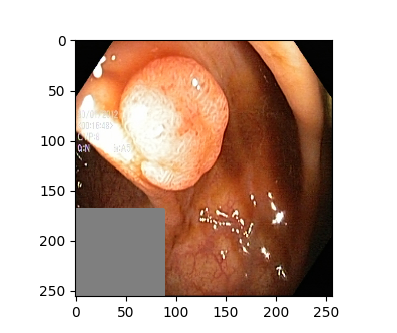
\includegraphics[width=\textwidth]{methodology/figures/masked_img.png}
    \caption[Hate to be this guy]
    {{\small Image the autoencoder receives as an input }}    
    \label{fig:AErec}
\end{subfigure}
\qquad
\begin{subfigure}[b]{0.42\textwidth}  
    \centering 
    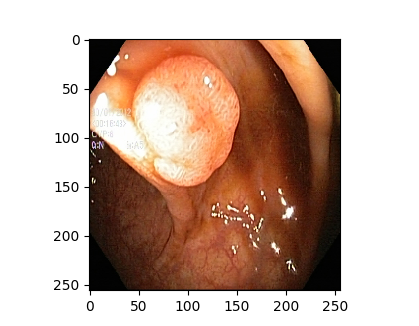
\includegraphics[width=\textwidth]{methodology/figures/whole_img.png}
    \caption[Hate to be this guy]%
    {{\small The missing part the autoencoder tries to replicate}}    
    \label{fig:AErep}
\end{subfigure}
\caption[Hate to be this guy]
{\small A standard image taken in by the autoencoder} 
\label{fig:AEmasks}
\end{figure*}

The next step before training is to cut the images according to the mask provided. Figure \ref{fig:AErec} shows what the finished masking looks like, and \ref{fig:AErep} shows what we want to achieve after training.

We feed \ref{fig:AErep} into the autoencoder consisting of convolutional layers, leakyReLu layers, and a tanh layer.
\todo{more}
\todo{remember to talk about loss}


\subsection{Generative adversarial network}
The gan used the same generator discriminator elements as the Goodfellow gan, but does not take in noise\todo{the best version does}


\subsection{Transfer learning classifier}
The dataset we are making with our generators needs to be classified. 

The classifier we use is based on the idea of reusing networks we already know apply well to the real world.
We have made a classifier that, by default, use one of the pretrained networks provided by the Keras framework.

\begin{table}[h]
\caption{Datasets provided by keras}
\begin{center}
\small
\begin{tabular}{llllll}
\toprule
\multicolumn{1}{c}
{Model}             & Size   & Top-1 Accuracy & Top-5 Acc & Parameters  & Depth \\
\midrule
Xception          & 88 MB  & 0.790          & 0.945          & 22,910,480  & 126   \\
VGG16             & 528 MB & 0.713          & 0.901          & 138,357,544 & 23    \\
VGG19             & 549 MB & 0.713          & 0.900          & 143,667,240 & 26    \\
ResNet50          & 98 MB  & 0.749          & 0.921          & 25,636,712  & -     \\
ResNet101         & 171 MB & 0.764          & 0.928          & 44,707,176  & -     \\
ResNet152         & 232 MB & 0.766          & 0.931          & 60,419,944  & -     \\
ResNet50V2        & 98 MB  & 0.760          & 0.930          & 25,613,800  & -     \\
ResNet101V2       & 171 MB & 0.772          & 0.938          & 44,675,560  & -     \\
ResNet152V2       & 232 MB & 0.780          & 0.942          & 60,380,648  & -     \\
ResNeXt50         & 96 MB  & 0.777          & 0.938          & 25,097,128  & -     \\
ResNeXt101        & 170 MB & 0.787          & 0.943          & 44,315,560  & -     \\
InceptionV3       & 92 MB  & 0.779          & 0.937          & 23,851,784  & 159   \\
InceptionResNetV2 & 215 MB & 0.803          & 0.953          & 55,873,736  & 572   \\
MobileNet         & 16 MB  & 0.704          & 0.895          & 4,253,864   & 88    \\
MobileNetV2       & 14 MB  & 0.713          & 0.901          & 3,538,984   & 88    \\
DenseNet121       & 33 MB  & 0.750          & 0.923          & 8,062,504   & 121   \\
DenseNet169       & 57 MB  & 0.762          & 0.932          & 14,307,880  & 169   \\
DenseNet201       & 80 MB  & 0.773          & 0.936          & 20,242,984  & 201   \\
NASNetMobile      & 23 MB  & 0.744          & 0.919          & 5,326,716   & -     \\
NASNetLarge       & 343 MB & 0.825          & 0.960          & 88,949,818  & -        \\   
\bottomrule
\end{tabular}
\end{center}
\label{tab:Kaeras_app}
\end{table}

Table \ref{tab:Kaeras_app} shows the pretrained networks available to load in the Keras framework. 
When training we did some extra steps at the end, namely added global average pooling and a fully connected layer with the desired number of outputs (usually eight classes, and eight outputs)




\section{Describe project}
Here i am going to explain the projects
\section{Summary}
At this point, we have described the reasoning behind using python, tensorflow and Keras for our machine learning. 
After this we looked into the filters used for training our models, and what type of preprocessing we wanted to do in addition to the inpainting. We looked at the advantages and disadvantages of preprocessing the Trest data, as opposed to just preprocessing the training data.

We then went more in-depth into how the three main programs were built up, and how they differ from their original sources.
First, we looked at the preprocessing methods, AE and GAN. We looked at how they learned from the samples, and we went more in-depth talking about the crucial layers for each model.

At last, we ended up giving a summary of the project as a whole, following a the Kvasir dataset from its original source into the generation of the six new datasets, and how each one of them was classified with all the different parameters to show the dataset-specific rate of success.

 
